
\chapter{Configurazione Router}

\section{Overview della configurazione}

In questo capitolo andremo a connettere il router 4g alla rete vpn e aggiungere le opportune regole in modo che il traffico proveniente dall'host domotico sia indirizzato verso la VPN

\section{Introduzione a Luci}

L'interfaccia grafica dovrebbe essere gia' installata e raggiungibile, in caso contrario puo' essere installata e configurata seguendo la guida ufficiale di \it{OpenWrt} \cite{install-luci}.

% TODO la figura non sta al posto suo
\begin{figure}[h!]
    \centering

    \begin{subfigure}{0.5\textwidth}
        \centering
        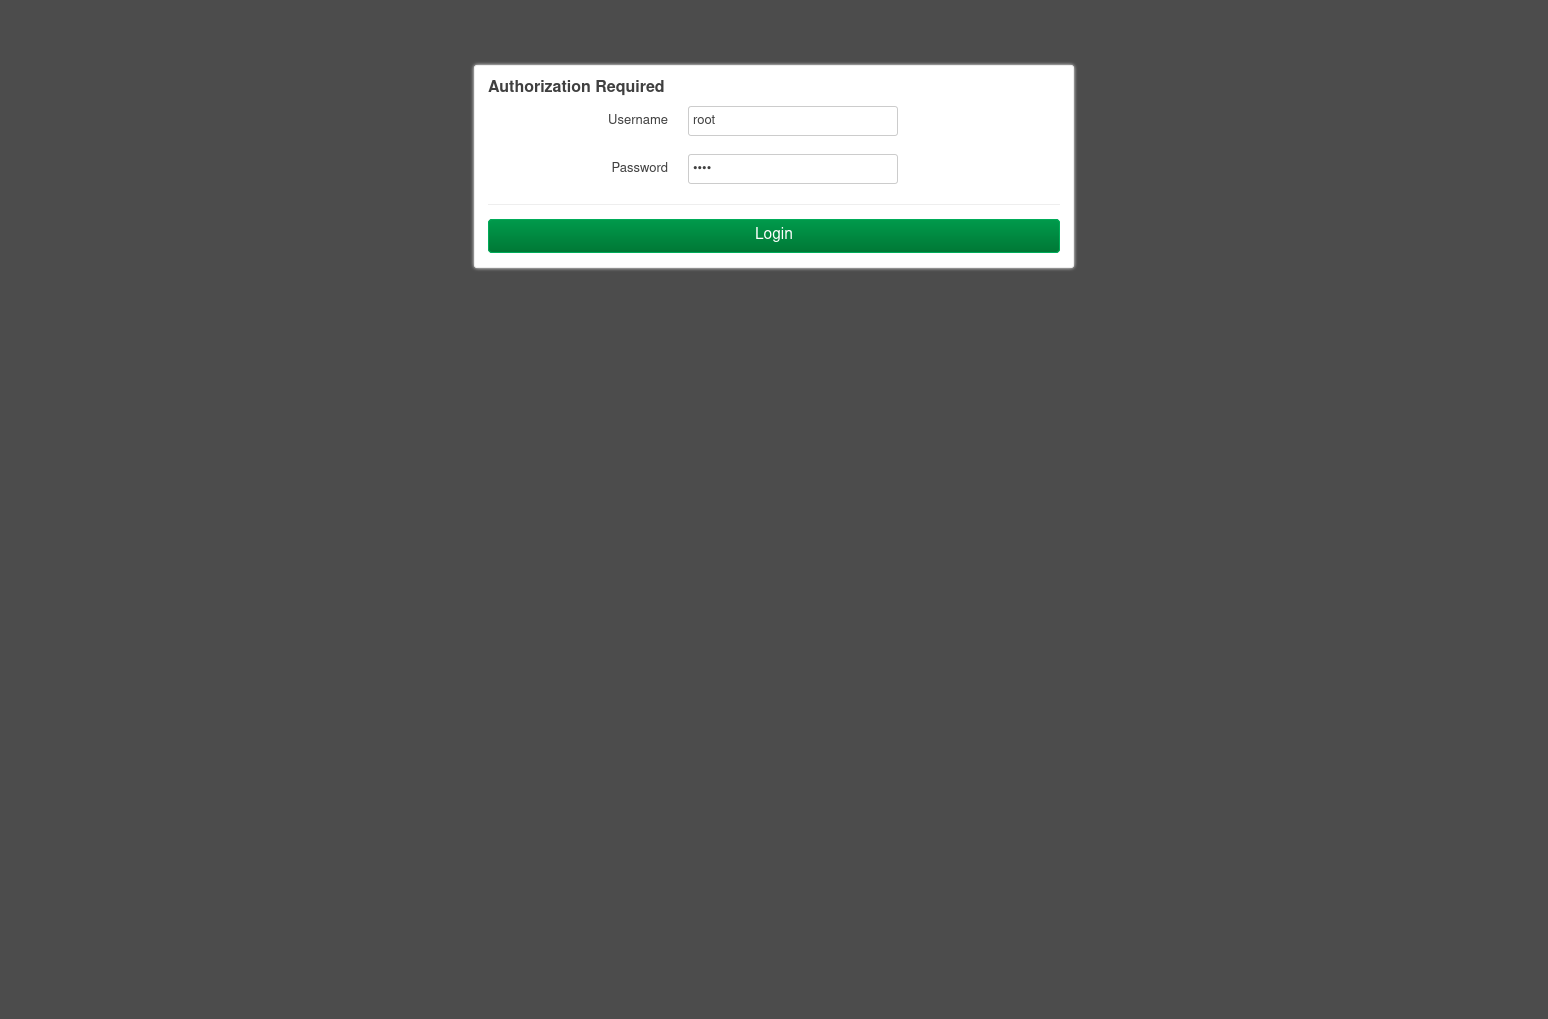
\includegraphics[height=0.6\linewidth]{immagini/LuCI_login}
        \caption{Login page}
        \label{fig:luci-login}
    \end{subfigure}%
    \hfill
    \begin{subfigure}{0.5\textwidth}
        \centering
        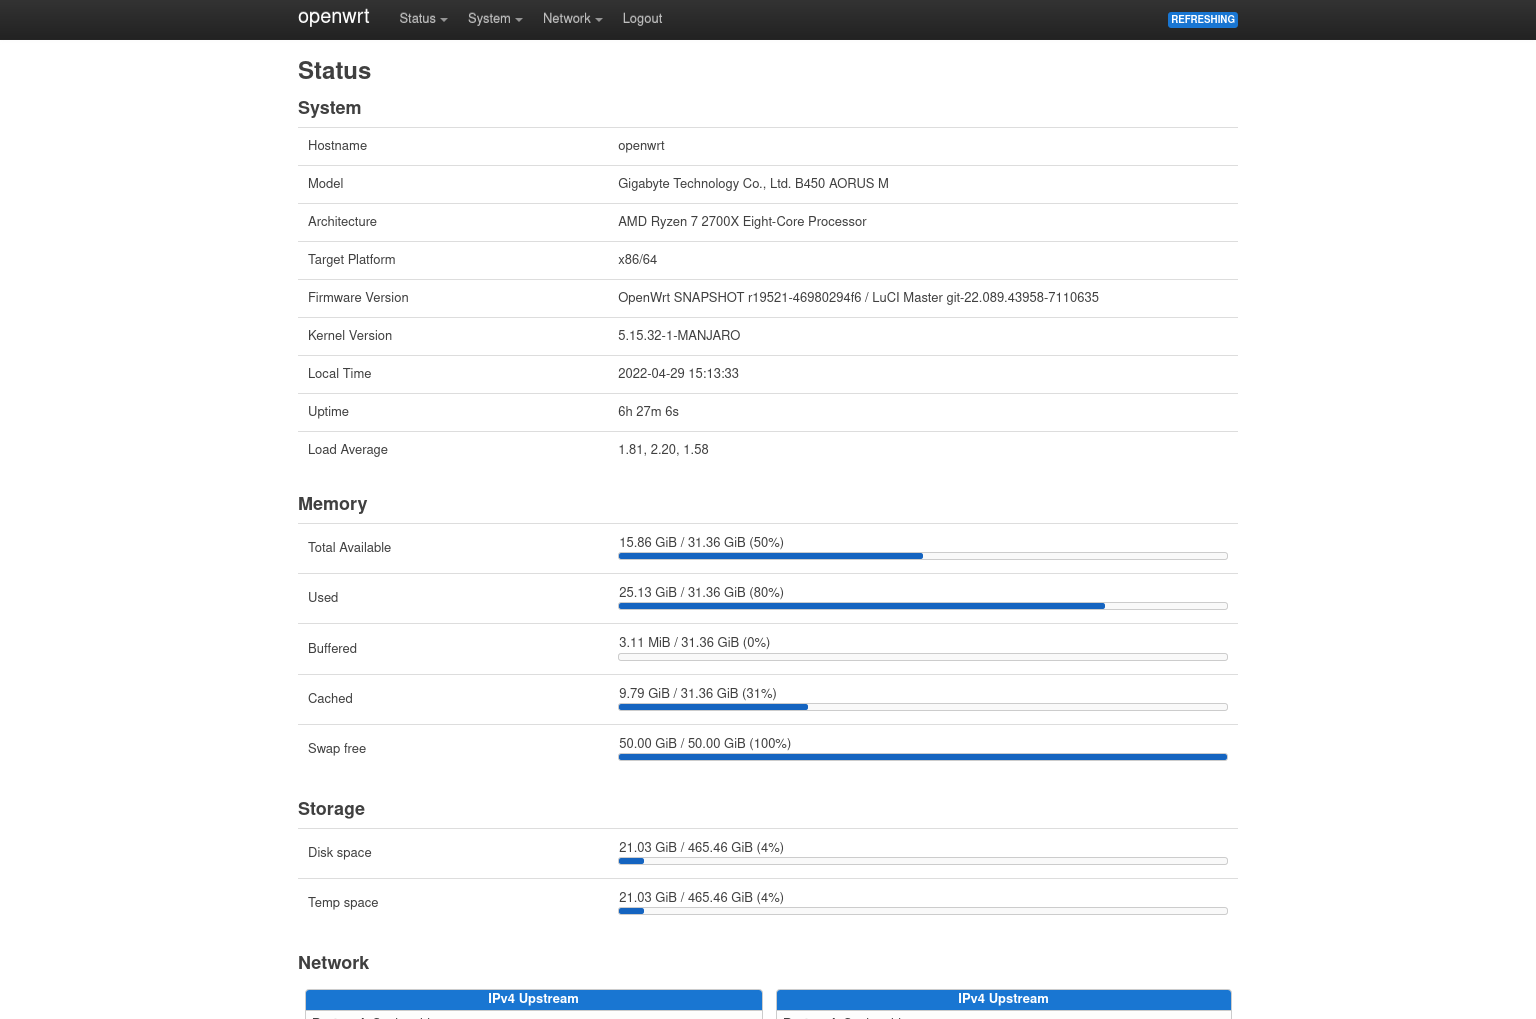
\includegraphics[height=0.6\linewidth]{immagini/LuCI_status}
        \caption{Status page}
        \label{fig:luci-status}
    \end{subfigure}%

    \begin{subfigure}{0.5\textwidth}
        \centering
        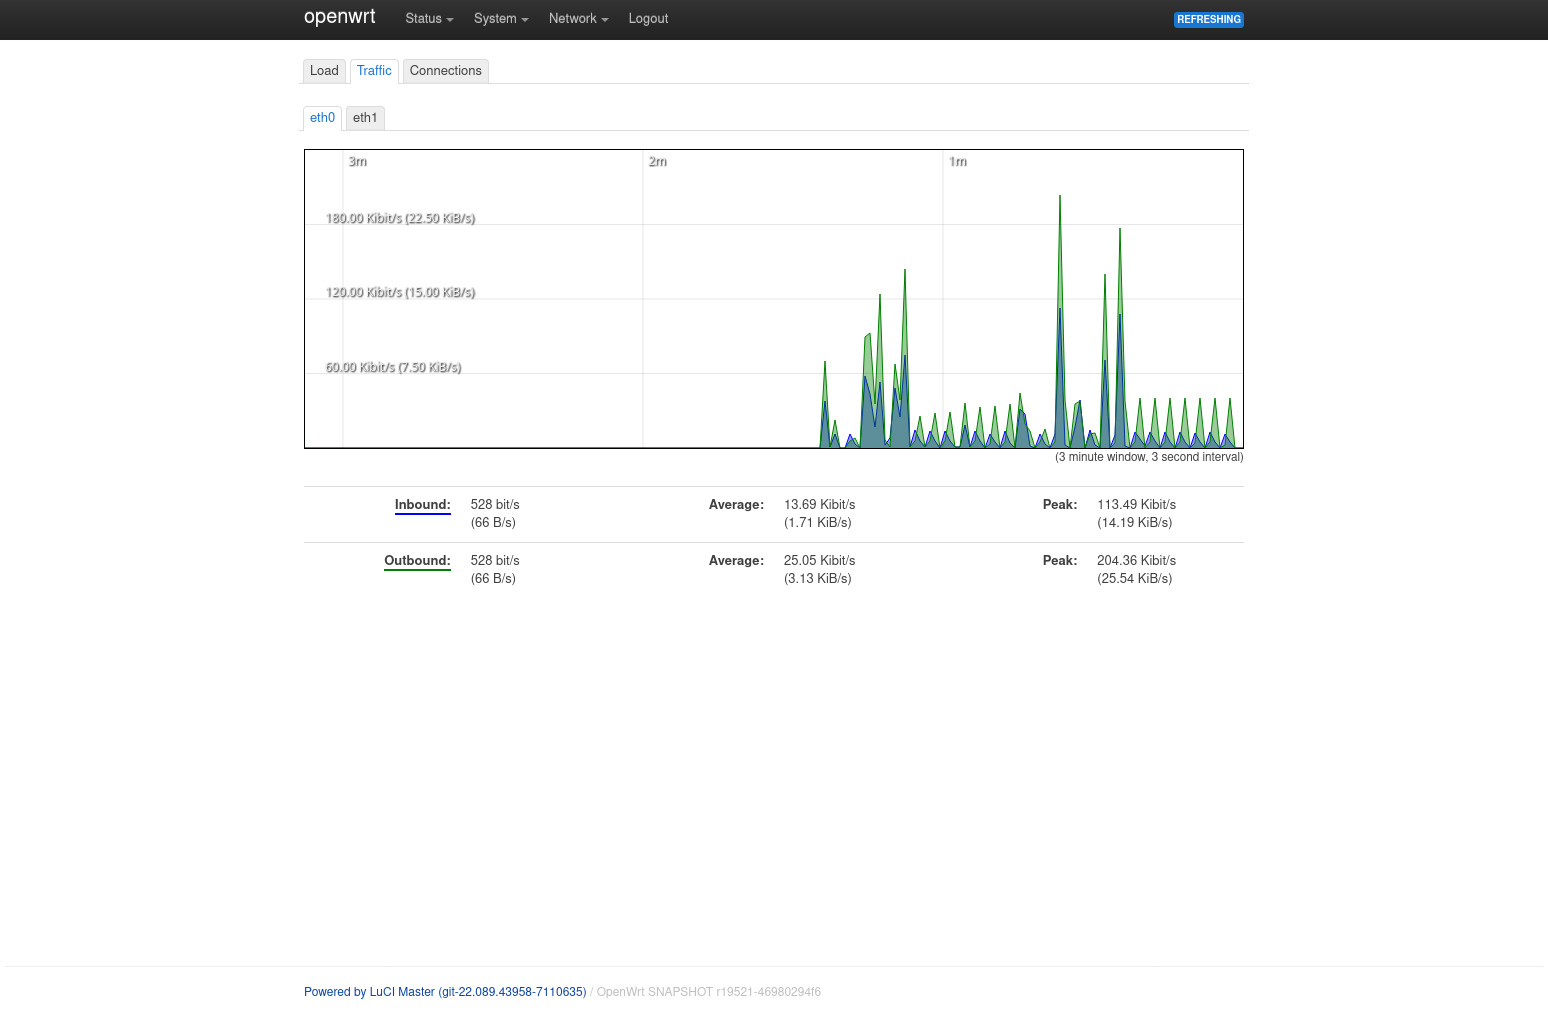
\includegraphics[height=0.6\linewidth]{immagini/LuCI_graphs}
        \caption{Graphs page}
        \label{fig:luci-graphs}
    \end{subfigure}%
    \hfill
    \begin{subfigure}{0.5\textwidth}
        \centering
        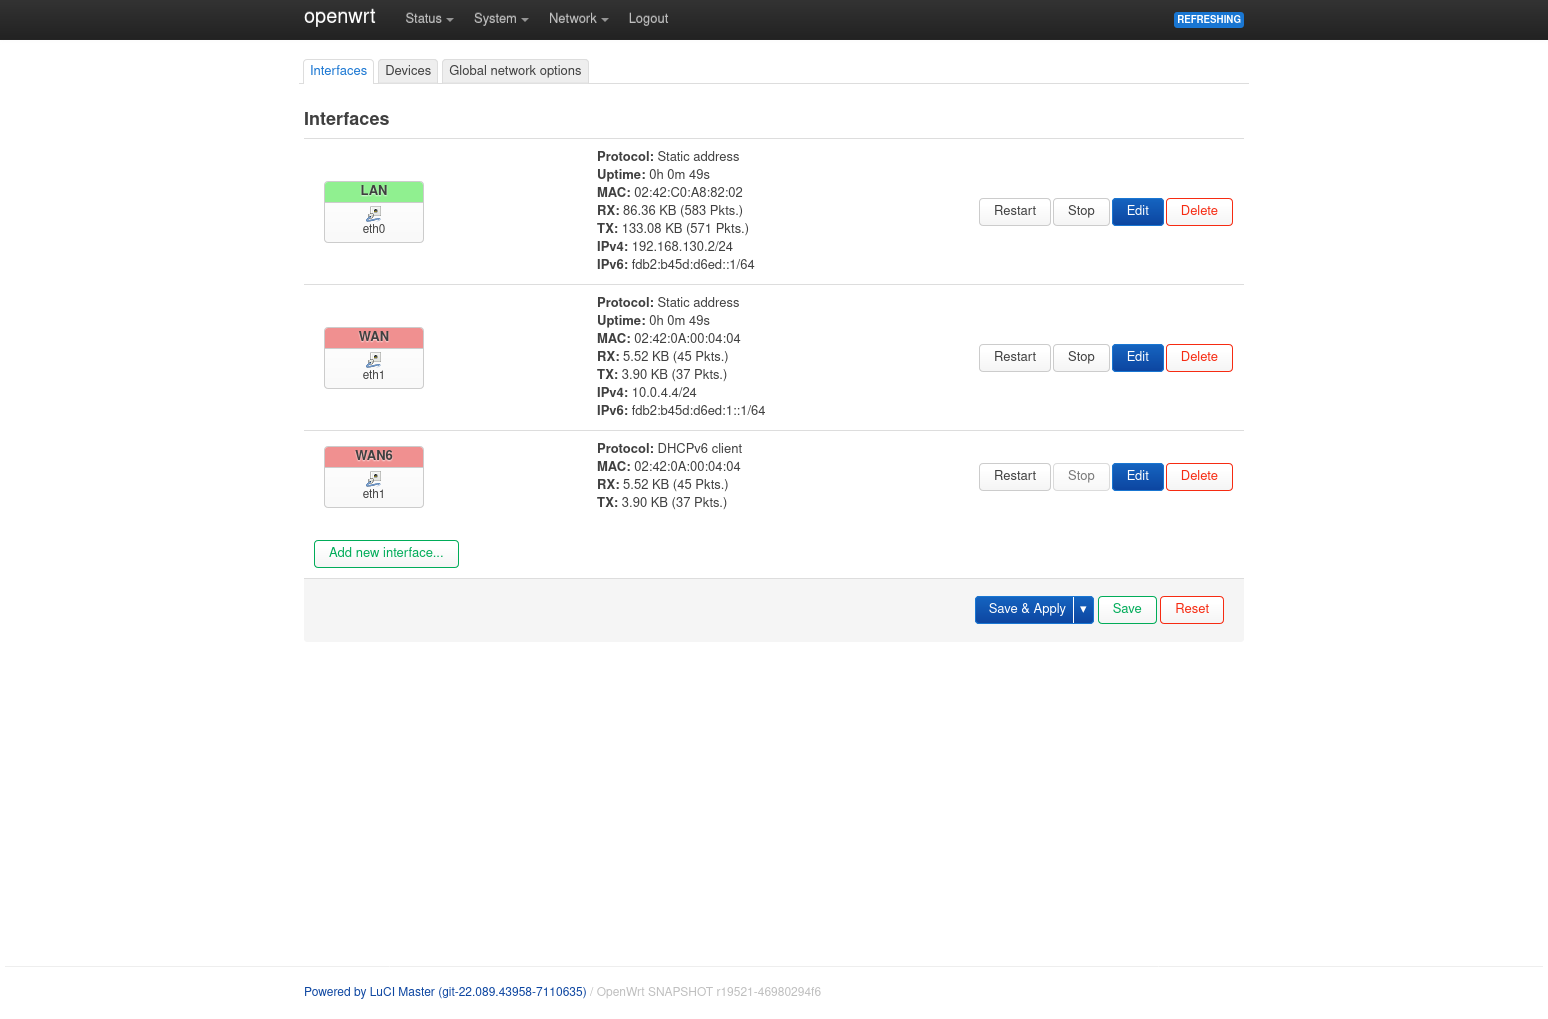
\includegraphics[height=0.6\linewidth]{immagini/LuCI_interfaces}
        \caption{Interfaces page}
        \label{fig:luci-graphs}
    \end{subfigure}%
    \caption{Interfaccia grafica LuCI}
\end{figure}

Le credenziali di default sono \code{Username:root} \code{Password:root}, come mostrato in fig. \ref{fig:luci-login}.

L'homepage, fig. \ref{fig:luci-status}, mostra un riepilogo dello stato del router, ad esempio sono presenti: informazioni sull'hardware, informazioni sulla memoria e storage, sono presenti inoltre informazioni riassuntive sulle interfacce di rete e sul \it{DHCP}.

L'interfaccia e' estensiva e permette di configurare quasi ogni aspetto del funzionamento del router, compreso il firewall, il \it{DHCP}, i processi in esecuzione, etc. 

\section{Accesso ssh al Router}

Oltre all'interfaccia grafica \it{LuCI} si puo' accedere al router tramite ssh.

\begin{bashcode}{Router 4g}{}
BusyBox v1.35.0 (2022-04-24 21:09:51 UTC) built-in shell (ash)
    _______                     ________        __
    |       |.-----.-----.-----.|  |  |  |.----.|  |_
    |   -   ||  _  |  -__|     ||  |  |  ||   _||   _|
    |_______||   __|_____|__|__||________||__|  |____|
            |__| W I R E L E S S   F R E E D O M
    -----------------------------------------------------
    OpenWrt SNAPSHOT, r19521-46980294f6
    -----------------------------------------------------
\end{bashcode}

Non esiste un account utente quindi viene effettuato il login come root.

\section{Creazione della configurazione e test}

Si devono seguire gli step descritti in sezione \ref{sec:client_keys}, quindi creare la certificate request e firmarla nel \it{server CA}. Per poi usare lo script creato in sezione \ref{sec:script_client} per costruire il file di configurazione:

\begin{bashcode}{Server}{}
$ ./make_config.sh router
\end{bashcode}

Dopodiché si deve spostare il file \code{router.ovpn} dal \it{Server} al \it{Router 4g}, supponiamo di averlo copiato nella cartella \code{/configs}. 

Di default non e' presente \it{OpenVPN} nel \it{Router 4g}, lo si puo' installare con:

\begin{bashcode}{Router 4g}{}
$ opkg update
$ opkg install openvpn
\end{bashcode}

Ora possiamo avviare il client openvpn:

\begin{bashcode}{Router 4g}{}
$ openvpn --config /configs/router.ovpn
2022-04-29 17:26:37 OpenVPN 2.5.6 x86_64-openwrt-linux-gnu [SSL (mbed TLS)] [LZ4] [EPOLL] [MH/PKTINFO] [AEAD]
[...]
2022-04-29 17:26:37 VERIFY EKU OK
2022-04-29 17:26:37 VERIFY OK: depth=0, CN=server
2022-04-29 17:26:37 Control Channel: TLSv1.2, cipher TLS-ECDHE-RSA-WITH-AES-256-GCM-SHA384, 2048 bit key
2022-04-29 17:26:37 [server] Peer Connection Initiated with [AF_INET]10.0.4.2:1194
2022-04-29 17:26:37 net_addr_ptp_v4_add: 10.8.0.10 peer 10.8.0.9 dev tun0
2022-04-29 17:26:37 Initialization Sequence Completed
\end{bashcode}

Se il file di configurazione e' stato creato correttamente si vedra' il messaggio \\\code{Initialization Sequence Completed}.

Comparira' inoltre l'interfaccia \code{tun0} a cui e' stato assegnato l'indirizzo \code{10.8.0.10}. 

\section{Abilitazione del Client-to-Client nel server OpenVPN}

Il \it{Router 4g} fa parte della rete VPN ma non puo' raggiungere tutti gli host della rete VPN, infatti:

\begin{bashcode}{Router 4g}{}
$ ping -c2 10.8.0.1                     # server openvpn
PING 10.8.0.1 (10.8.0.1): 56 data bytes
64 bytes from 10.8.0.1: seq=0 ttl=64 time=0.285 ms
64 bytes from 10.8.0.1: seq=1 ttl=64 time=0.208 ms

--- 10.8.0.1 ping statistics ---
2 packets transmitted, 2 packets received, 0% packet loss
round-trip min/avg/max = 0.208/0.246/0.285 ms

$ ping -c2 10.8.0.6                     # client1
PING 10.8.0.6 (10.8.0.6): 56 data bytes

--- 10.8.0.6 ping statistics ---
2 packets transmitted, 0 packets received, 100% packet loss
\end{bashcode}

